\chapter{Existing solutions to the problem of tracklet building}\label{chap:existing_solutions}

\section{k-d trees}\label{sec:kd_trees}
	
	k-dimensional trees (k-d trees) are a hierarchical data structure that recursively partitions both the set of data points and the space in which they reside into smaller subsets and subspaces. Each node in a k-d tree represents a partial region of the whole space and a set of points contained in the region \citep{}.
	
	Complexity of k-d trees is similar, or identical in some cases, to other tree data structures. For example, adding a point into a balanced k-d tree takes $O(log\ n)$ time and removing a point from a balanced k-d tree takes $O(log\ n)$ time as well. There are several approaches to constructing a k-d tree, such as finding a median among points (with complexity $O(n)$), sorting all points (with complexity $O(log\ n)$) or sort a fixed number of randomly selected points.

\subsection{Efficient intra- and inter-night linking of asteroid detections using kd-trees}\label{subsec:intra_inter}

	The main focus of the paper is the description of then under development Panoramic Survey Telescope and Rapid Response System (Pan-STARRS) creating the first fully automated Moving Object Processing System (MOPS) in the world. The paper describes the capabilities of the system in areas such as identification of detection of moving objects in our solar system and linking of those detections within and between nights, attributing those detections to catalogued objects, calculating initial and differentially corrected orbits and orbit identification. Further, it illustrates k-d tree algorithms as suitable for linking of objects within and between nights. The paper contains the description of their own pseudo-realistic simulation of the Pan-STARRS survey strategy and shows the results on both simulated and real data sets.
	
\subsubsection{Pan-STARRS}
	
	The paper describes future goals of Pan-STARRS - obtaining 2 images per night of each Solar System survey field and using these images to distinguish between real and false detections and to separate stationary and moving transient near-Earth objects (NEOs). Since submissions to the Minor Planet Center (MPC, see Chapter \ref{chap:results}, Section \ref{sec:mpc}) need to have a high probability of the submitted object to be real, obtaining the object several more times during following nights provides sufficient observations with which to calculate an orbit and verify the realness of each set of detections.
	
\subsubsection{Pan-STARRS MOPS}
	
	However, before an image can be processed by MOPS, it must be first passed through Image Processing Pipeline that removes cosmic rays and other clutter, aligns and digitally combines the images into a single image. The combination of these single images is possible and is done to create a static-sky image that is subtracted from the currently edited master image in order to produce an image containing only transient sources and noise. The resulting image is then searched for asteroids and comets\; pairs of subtracted images are analysed similarly. The preprocessing phase ends with all the identified sources from both images, along with their metadata (time, trail length, axis orientation, flux, etc.), being passed to the MOPS.
	
	The first step, linking intra-night detections of spatially and temporally close objects, which, in addition, have fixed speed among multiple detections, into tracklets, is being done by comparing expected and detected trail length and orientation. Only the objects which pass through this filter are combined into tracklets. The second step is the inter-night linking of tracklets into tracks, which are basically just collections of tracklets. The tracks are verified by IOD (see Chapter \ref{chap:object_dynamics}, Section \ref{sec:init_orbit_det}) and OD. The complexity of the linkingincreases like $\rho^2$, where $\rho$ is the number of detections/deg$^2$. This can be solved by employing k-d trees to reduce the complexity that increases like $\rho\ log\ \rho$.
	
	\begin{figure}[H]
	\centering
	  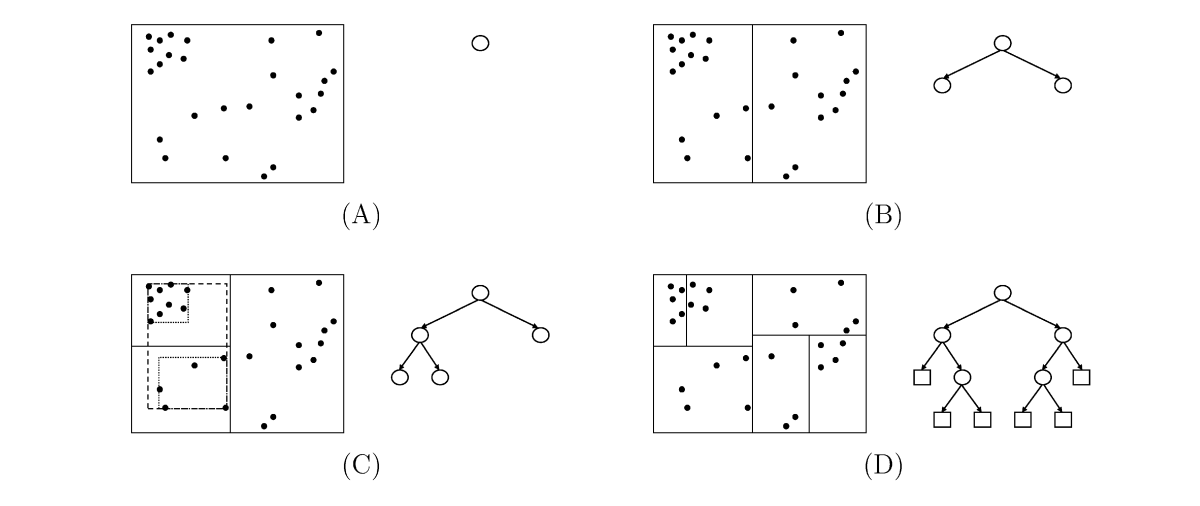
\includegraphics[width=10cm]{images/kd_tree}
		  \caption{k-d tree schematic.}
	  \label{fig:kd_tree}
	\end{figure}
	
	The k-d tree is created from top to down, having full image as the root node. At each level the data in form of points is used to create a bounding box which is then saved in the corresponding node. The points are then split into two disjoint sets at the widest dimension of the node and bounding boxes are created and assigned again. The recursion of creating nodes is stopped when the currently created node owns less than pre-determined number of points and such node is marked as a leaf node. The construction process is illustrated in Figure \ref{fig:kd_tree}.
	
	Searching for spatially close nodes is done by descending the tree depth first and searching for points within a radius from a given point of query. If the algorithm finds a node that falls out of the radius, due to the nature of k-d tree, the algorithm stops because it is guaranteed that each child of the node will fall out of the radius as well. If the algorithm reaches a leaf node, the points in it are tested for the distance from the point of query and eventually added to the results. The algorithm is extended by another constraint - temporal significance. In the paper, they consider each detection as the start of a potential tracklet and look at temporally subsequent detections to judge their relevance and add them to the tracklet. Time is added to the k-d tree as a third dimension. The result of having time as the third dimension is illustrated in Figure \ref{fig:kd_tree_time} as a cone which spread is controlled by the maximum allowed speed.
	
	\begin{figure}[H]
	\centering
	  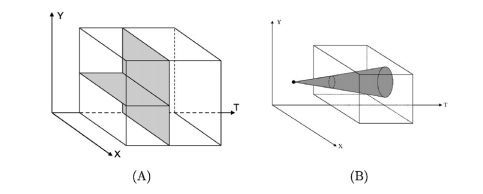
\includegraphics[width=10cm]{images/kd_tree_time}
		  \caption{k-d tree temporal search.}
	  \label{fig:kd_tree_time}
	\end{figure}
	
	Inter-night linking is out of scope of this thesis, similarly to creation of synthetic data and their description can be found in the paper.

\section{Uniform linear motion detection}\label{sec:linear_motion}
	
	

\subsection{Optical observation, image-processing, and detection of space debris in GEO}\label{subsec:linear_geo}